\lfoot{Autor: Tobias Perny}
\subsubsection{I2C}
\label{subsec:I2C}
I2C, Inter Integrated Circuit, ist ein Datenbus bestehend aus zwei Leitungen, einer Datenleitung und einer Taktleitung. Der I2C-Bus eignet sich zur Datenübertragung über kurze Entfernung, beispielsweise auf derselben Platine.

\begin{wrapfigure}{r}{0.2\textwidth}
  \begin{center}
    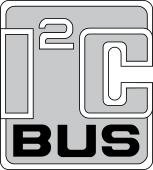
\includegraphics[width=0.2\textwidth]{images/i2c}
  \end{center}
  \caption{Logo von i2c \cite{PERT.CH2-i2c.logo}}\label{Fig:imgi2cLogo}
\end{wrapfigure}

\textbf{Grundlagen\newline}
Der I2C-Bus baut auf einem Master-Slave System auf, dass bedeutet es existiert mindestens ein Master und bis zu 127 Slaves auf einem Bus. I2C ist unter anderem ein Multi-Master-Bus, was bedeuted es können mehrere Master zur selben Zeit existieren und der Bus ist noch Lauffähig.
Alle Teilnehmer am Bus erhalten eine eindeutige Adresse. Ein Master kann mithilfe dieser Adresse Daten senden oder empfangen.
\nextline
\textbf{Beispiel\nextline}
Eine Beispielhafte Kommunikation könnte folgendermaßen aussehen:
\nextline
Auf einem I2C-Bus liegt ein Mikrocontroller mit der Adresse 00 und ein Beschleunigungssensor mit der Adresse 01. Der Mikrocontroller übernimmt die Rolle des Masters und der Sensor ist der sogenannte Slave. Nun möchte man Daten aus dem Sensor auslesen. Der Microkontroller prüft ob der Bus „frei“ ist, also ob niemand anderer die Leitung belegt. Dies ist nicht der Fall also sendet der Master eine Nachricht bestehend aus der Zieladresse (in diesem Fall „01“) und teilt dem Slave mit ob Daten gesendet oder empfangen werden sollen. Nun sendet der Slave die Daten an den Controller bis die kommunikation vom Master beendet wird.


\clearpage % DO NOT REMOVE